\documentclass[12pt,a4paper]{article}
\usepackage[spanish]{babel} % Corta palabras en espa~nol
\usepackage[utf8]{inputenc} % Escribir con acentos, ~n...
\usepackage{eurosym} % s´ımbolo del euro
\newcommand{\horrule}[1]{\rule{\linewidth}{#1}} % Create horizontal rule command with 1 argument of height
\usepackage{listings}             % Incluye el paquete listings
\usepackage{graphics,graphicx, float} %para incluir imágenes y colocarlas

\title{
\normalfont \normalsize 
\textsc{{\bf Aprendizaje Automatico (2018-2019)} \\ Grado en Ingeniería Informática \\ Universidad de Granada} \\ [25pt] % Your university, school and/or department name(s)
\horrule{0.5pt} \\[0.4cm] % Thin top horizontal rule
\huge Práctica 0 \\ % The assignment title
\horrule{2pt} \\[0.5cm] % Thick bottom horizontal rule

\includegraphics{images/logo.png}	
}

\author{Antonio Jesús Heredia Castillo} % Nombre y apellidos

\date{\normalsize\today} % Incluye la fecha actual

%----------------------------------------------------------------------------------------
% DOCUMENTO
%----------------------------------------------------------------------------------------

\begin{document}

\maketitle % Muestra el Título
\newpage %inserta un salto de página
\tableofcontents % para generar el índice de contenidos
\listoffigures
\newpage

\section{Parte 1}
\subsection{Leer la base de datos de iris que hay en scikit-learn}
En esta parte lo primero que realizaremos es leer de la base de datos iris para obtener tanto los datos de entrada como a la clase que pertenecen. Para ello usamos:
\begin{lstlisting}[language=Python]
iris = datasets.load_iris()
\end{lstlisting}
\subsection{Obtener las dos ultimas características y la clase}
De entrada guardo todos los datos en el mismo array, por si en un futuro los necesito tenerlos accesibles. Luego separo cada eje que usare en la grafica y la clase a la que pertenecen.
\begin{lstlisting}[language=Python]
array_datos = np.column_stack((iris.data[:, 2:],iris.target))
#inicializo variables que voy a usar
y_axis  = array_datos[:,1]
x_axis = array_datos[:,0]
target =  array_datos[:,2]\end{lstlisting}
\subsection{Visualizar los datos}
Para visualizar los datos, he realizado un bucle, el cual va comparando a que clase pertenece ese dato, para poner la etiqueta y el color correspondiente. Tambien los guardo de forma clasificada ya que en el siguiente apartado lo necesitare asi. 
\begin{lstlisting}[language=Python]
for pos in range(0,target.size):
    if(target[pos] == 0):
        plt.scatter(x_axis[pos], y_axis[pos], color='blue', 
        label="Clase 0" )
        clase_0 = np.append(clase_0, array_datos[pos:pos+1,
        [0,1,2]],axis=0)
    elif (target[pos] == 1):
        plt.scatter(x_axis[pos], y_axis[pos], color='red', 
        label="Clase 1")
        clase_1 = np.append(clase_1, array_datos[pos:pos+1,
        [0,1,2]],axis=0)
    else:
        plt.scatter(x_axis[pos], y_axis[pos], color='green', 
        label="Clase 2")
        clase_2 = np.append(clase_2, array_datos[pos:pos+1,
        [0,1,2]],axis=0)\end{lstlisting}
La grafica obtenida la podemos ver en Figura \ref{figura1}
\begin{figure}[H]  %con el [H] le obligamos a situar aquí la figura
\centering
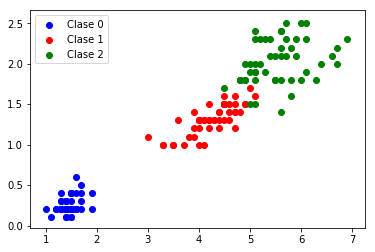
\includegraphics{images/graficaPuntos.png}  %el parámetro scale permite agrandar o achicar la imagen. En el nombre de archivo puede especificar directorios
\caption{Grafica de puntos de los datos. (En el eje x se puede observar la penultima columna de iris y en el eje y la ultima columna)}
\label{figura1}
 
\end{figure}
\section{Parte 2}
\subsection{Separar en training y test conservando la proporción.(80/20)}
Para separar los datos en entrenamiento y test yo lo he realizado de la siguiente forma. Primero creo dos arrays, uno para el test y otro para el entrenamiento. Y lo que hare es sacar de forma aleatoria el 20\% de cada clase y el dato que meto en el array de test lo elimino del array en el que estaba. Asi cuando saquemos el 20\% en el array original quedara el 80\% de los datos que usaremos para el entrenamiento. Por ejemplo para la clase 0 lo realizo de la siguiente forma:
\begin{lstlisting}[language=Python]
tam = int(len(clase_0)*0.2)
for pos in range(0,tam):
    rand = random.randrange(len(clase_0))
    test = np.append(test, clase_0[rand:rand+1,[0,1,2]],axis=0)
    clase_0 = np.delete(clase_0,[rand],axis=0)
\end{lstlisting}
Se puede ver que elijo un elemento de forma aleatoria, lo añado al array de test y lo elimino de array en el que estaba. Esto lo realizo para todos los elementos de cada clase de forma independiente para preservar la proporción. Luego con los datos que nos "sobran", los añadimos al array de entrenamiento de la siguiente forma:
 \begin{lstlisting}[language=Python]
tam = int(len(clase_0)*0.2)
for pos in range(0,tam):
    rand = random.randrange(len(clase_0))
    test = np.append(test, clase_0[rand:rand+1,[0,1,2]],axis=0)
    clase_0 = np.delete(clase_0,[rand],axis=0)
\end{lstlisting}
No he querido sobrecargar la salida de datos en la consola y por lo tanto no he mostrado todos los datos. Solo he mostrado la cantidad de datos de cada array. No obstante se puden ver los datos desde Spyder, en el explorador de variables.
\section{Parte 3}
\subsection{Obtener 100 valores equiespaciados desde 0 a 2$\pi$}
Para realizar este apartado usare el comando linespacae que incluye numpy.
\begin{lstlisting}[language=Python]
valores =np.linspace(0,2*math.pi,num=100)
\end{lstlisting}
\subsection{Obtener los valores para sen(x), cos(x) y sen(x)+cos(x) de los 100 valores anteriores}
Para esto recorreremos los 100 valores que obtuvimos en el apartado anterior y evaluaremos las funciones de sen, cos y la suma  de ambas y las guardaremos en vectores diferentes.
\begin{lstlisting}[language=Python]
for pos in range(0,valores.size):
    valores_sin = np.append(valores_sin, math.sin(valores[pos])) 
    valores_cos = np.append(valores_cos, math.cos(valores[pos])) 
    valores_mix = np.append(valores_mix, 
    math.sin(valores[pos])+math.cos(valores[pos]))\end{lstlisting}
\subsection{Visualizar las tres curvas simultáneamente en el mismo plot( con lineas discontinuas en negro, azul y rojo}
Para eso uso el comando plot. Lo primero que le tenemos que pasar a plot es los valores del eje x. Despues debe ir los valores del eje y. Tambien indicaremos que queremos lineas discontinuas con ``- -'' y el color.
Tendremos una salida como la que se ve en la Figura \ref{figura2}.

\begin{figure}[H]  %con el [H] le obligamos a situar aquí la figura
\centering
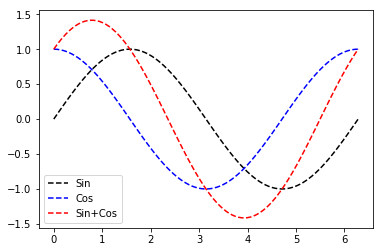
\includegraphics{images/graficaLineas.png}  %el parámetro scale permite agrandar o achicar la imagen. En el nombre de archivo puede especificar directorios
\caption{Grafico de lineas discontinuas.}
\label{figura2}
 
\end{figure}
\end{document}